\chapter{Processing di immagini a colori}
Tutti gli strumenti presentati nel capitolo precedente possono essere applicati con successo anche alle immagini a colori, occorre però prestare attenzione e scegliere con giudizio come trattare i diversi canali. In \ref{sec:color_model} abbiamo presentato diversi spazi colore, scegliere quello corretto per rappresentare i dati che vogliamo elaborare è fondamentale ai fini di ottenere un buon risultato.

\section{Color slicing}
Avere a disposizione un'immagine colorata ci permette di segmentare l'immagine non solamente considerando l'energia totale (valore del livello di grigio), ma anche in base al colore.

\subsection{Segmentare col modello HSI}
Il modo più ovvio per segmentare un'immagine è quello di passare al modello HSI, in questo modello infatti possiamo definire direttamente la tinta (H) che ci interessa e selezionare tutti i pixel che hanno una tinta vicina.

In certi casi può essere utile avere delle soglie anche sulla saturazione (S), in modo da avere degli algoritmi robusti quando si dovessero incontrare colori la cui tinta non è ben definita come i grigi. Mentre non si usa mai l'intensità che non porta alcuna informazione sul colore.

Quando si segmenta con questo spazio colore è necessario prestare attenzione alla definizione del modello stesso, siccome la hue è la distanza dal rosso in corrispondenza del rosso c'è un salto di continuità, questo significa che tinte percettivamente simili al rosso come il magenta avranno in realtà distanza massima da quest'ultimo. Se si devono segmentare oggetti rossi bisogna prendere in considerazione questa discontinuità.

\subsection{Segmentare col modello RGB}
Per segmentare con lo spazio colore RGB abbiamo bisogno di definire il colore medio degli oggetti che vogliamo evidenziare, il modo più comodo per fare questo è selezionare a mano un certo numero di pixel che sappiamo appartenere all'oggetto di interesse e computare poi la media.

Una volta stabilito il colore medio abbiamo bisogno di un modo per accettare o rifiutare altri colori. Nello spazio HSI questo era molto semplice, si definiva una soglia e si valutava se la distanza dalla tinta selezionata era maggiore o minore. Nel modello RGB invece possiamo definire una distanza geometrica tra il colore del pixel che stiamo analizzando e il colore target (questo perché i colori si trovano in un cubo).

Abbiamo tipicamente tre alternative per decidere se accettare o meno un pixel:
\begin{itemize}
	\item \textbf{cubo}: costruiamo un cubo intorno al colore target, tutti i pixel il cui colore cade dentro al cubetto saranno selezionati;
	\item \textbf{sfera}: si definisce una distanza di soglia, tutti i pixel il cui colore dista da quello target meno della soglia saranno accettati;
	\item \textbf{distanza di Mahalanobis}: è una distanza adattativa che tiene conto che alcune componenti di colore possano variare più di altre.
\end{itemize}

\subsubsection{Distanza di Mahalanobis}
Usare una sfera per segmentare prevede che ciascuna componente possa variare fino a una soglia massima uguale per tutte le componenti. Ci sono casi in cui la componente verde del target rimane molto stabile mente la componente rossa varia molto, usare un sfera in questo caso porterà per forza a errori.

Quando si selezionano i pixel target si calcola anche una matrice di covarianza, questa ci permette di descrivere il comportamento di una componente rispetto alle altre e genera un'area di accettazione dei pixel a forma di ellissoide ruotato in modo da rispettare la distribuzione dei pixel che abbiamo selezionato per definire il colore target.

\begin{wrapfigure}{l}{.6\linewidth}
	\centering
	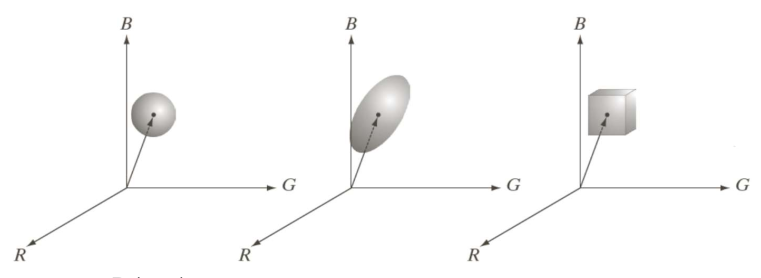
\includegraphics[width=.95\linewidth]{Picture/Color_Slicing}
\end{wrapfigure}
Nella figura sono rappresentate le diverse forme per definire la regione di accettazione dei pixel. Solo la distanza di Mahalanobis si adatta alla distribuzione dei pixel target.